%!TEX root = ../../../_main.tex
\section{Posets}
\label{sec:posets}

Posets are sets $M$ with a partial order $\leq$. In particular, there are pairs $(a,b) \in M \times M$ of distinct elements such that neither $a \leq b$ nor $a \geq b$. The following definitions and examples define this mire precisely.

\begin{defi}
	\typedlabel{defi:poset}
	Let $M$ be a set. A binary relation $\leq$ is called a \defword{partial order} over $M$, if for all $a,b,c \in M$ it satisfies the conditions
	\begin{enumerate}
		\item $a \leq a$ (\defword{reflexivity}),
		\item $a \leq b \wedge b \leq a \Rightarrow a=b$ (\defword{antisymmetry}) and
		\item $a \leq b \wedge b \leq c \Rightarrow a \leq c$ (\defword{transitivity}).
	\end{enumerate}
	In this case $(M,\leq)$ is called a \defword{poset}. If two elements $a \leq b \in M$ are immediate neighbors, i.e. there is no third element $c \in M$ with $a \leq c \leq b$ we say that $b$ \defword{covers} $a$.
\end{defi}

\begin{defi}
	A poset is called \defword{graded poset} if there is a map $\rho : M \to \nn$ such that for all $a,b \in M$ with $b$ covers $a$ we have $\rho(b) = \rho(a) + 1$. In this case $\rho$ is called the \defword{rank function} of the graded poset.
\end{defi}

\begin{defi}
	A poset is called \defword{directed poset}, if for any two elements $a,b \in M$ there is an element $c \in M$ with $a \leq c$ and $b \leq c$. It is called \defword{bounded poset}, if it has a unique minimal and maximal element, denoted by $\hat 0$ and $\hat 1$.
\end{defi}

\begin{defi}
	Let $(M,\leq)$ be a poset and $a,b \in M$. Then we call $\{ c \in M : a \leq c \leq b \}$ an \defword{interval} and denote it by $[a,b]_\leq$. The set $\{ c \in M : a < c < b \}$ is called an \defword{open interval} and is denoted by $(a,b)_\leq$. In both cases we can omit the $\leq$, if the relation is clear from context.
\end{defi}

\begin{defi}
	\typedlabel{defi:hasse-diagram}
	The \defword{Hasse diagram} of the poset $(M,\leq)$ is the graph obtained in the following way: Add a vertex for each element in $M$. Then add a directed edge from vertex $a$ to $b$ whenever $b$ covers $a$.
\end{defi}

\begin{exam}
	Suppose we have an arbitrary set $M$. Then the powerset $\mathcal P (M)$ can be partially ordered by the subset relation, so $(\mathcal P (M), \subseteq)$ is a poset. Indeed this poset is always graded with the cardinality function as rank function. In Figure \ref{fig:poset-xyz-subsets} we see the Hasse diagram of this poset with $M = \{x,y,z\}$.

	\begin{figure}[ht]
		\centering
		%!TEX root = ../../_main.tex
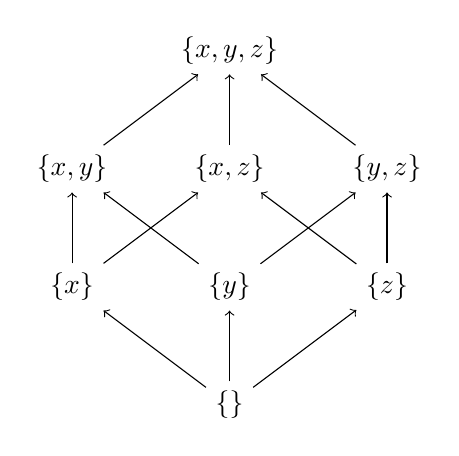
\begin{tikzpicture}
	\tikzstyle{every node}=[]
	\tikzstyle{relation}=[->]

	\node (xyz) at (0,0) {$\{x,y,z\}$};
	\node (xy) at (-2,-1.5) {$\{x,y\}$};
	\node (xz) at (0,-1.5) {$\{x,z\}$};
	\node (yz) at (2,-1.5) {$\{y,z\}$};
	\node (x) at (-2,-3) {$\{x\}$};
	\node (y) at (0,-3) {$\{y\}$};
	\node (z) at (2,-3) {$\{z\}$};
	\node (0) at (0,-4.5) {$\{\}$};
	\draw[relation] (0) -- (x);
	\draw[relation] (0) -- (y);
	\draw[relation] (0) -- (z);
	\draw[relation] (x) -- (xy);
	\draw[relation] (x) -- (xz);
	\draw[relation] (y) -- (xy);
	\draw[relation] (y) -- (yz);
	\draw[relation] (z) -- (xz);
	\draw[relation] (z) -- (yz);
	\draw[relation] (xy) -- (xyz);
	\draw[relation] (xz) -- (xyz);
	\draw[relation] (yz) -- (xyz);
\end{tikzpicture}
		\caption{Hasse diagram of the set of all subsets of $\{x,y,z\}$ order by the subset relation}
		\label{fig:poset-xyz-subsets}
	\end{figure}
\end{exam}

\begin{defi}
	\typedlabel{defi:direct-product-of-posets}
	Let $(M_i, \leq_i), i = 1,\ldots,n$ be a finite set of posets. We call the poset
	$$ (M_1 \times \ldots \times M_n,\leq) \textrm{ with } (a_1,\ldots,a_n) \leq (b_1,\ldots,b_n) \iff a_i \leq_i b_i \textrm{ for } i=1,\ldots,n $$
	a \defword{direct product of posets} and denote it by $(M_n, \leq_n) \times \ldots \times (M_n, \leq_n)$.
\end{defi}